\section{Subsystem visual evidence and independent software checks}
\label{app:des-visual-tests}
This appendix records newly run offline checks and illustrations made from existing project data. It supplements the Design explanations; the integrated qualification tests against the proposal remain in Results. The evidence scripts use the current processing modules, record source and input SHA-256 hashes, and write their outputs into this revision's \texttt{Evidence} directory. No training or physical motion was performed. Diagnostic settings are stated explicitly rather than inherited silently from server defaults.

\subsection{Actual capture variation and input resolution}
The three camera-roll inputs in Figure~\ref{fig:des-seg-variation} are \texttt{WIN\_20261028\_23\_23\_30\_Pro.jpg}, \texttt{WIN\_20261028\_23\_28\_34\_Pro.jpg} and \texttt{WIN\_20261028\_23\_32\_40\_Pro.jpg}. Each stored image is $3264\times2448$ pixels. The page visibly contains three handwritten text rows. Automatic axis decisions were retained, including the failure in the third capture. The observed crop counts were 4, 3 and 28, respectively. Shadows are visually different, but neither lux levels nor physical angles were measured. These observations therefore explain a design limitation rather than qualifying operation across a specified lighting range.

The native Owen01 page ($2448\times3264$) produced 20 crops for 20 labelled lines. A separate exploratory bench first fitted each of three original pages inside $1600\times1600$ pixels. From each reduced page it produced an unchanged view, a synthetic left-to-right multiplier from 0.42 to 1.00, a synthetic $+3^\circ$ rotation using bicubic interpolation on an expanded white canvas, and a quarter turn. Each was passed through the same automatic axis and segmentation functions. Table~\ref{tab:des-resample-cases} retains every case, including unsuccessful ones.
\begin{table}[!htbp]\centering\small
\begin{tabular}{lrrrrr}\hline
Page & Label lines & Reduced & Gradient & $+3^\circ$ & $90^\circ$ \\\hline
Owen & 20 & 19 & 20 & 11 & 19 \\
Dylan & 24 & 24 & 24 & 25 & 24 \\
Yeukita & 26 & 26 & 26 & 26 & 26 \\
\hline\end{tabular}
\caption{Exploratory crop counts after extra input reduction and digital perturbation. Equal counts do not establish correct ink ownership.}
\label{tab:des-resample-cases}
\end{table}
The reduced Owen case produced 19 crops and lost the usable first-line crop, whereas the native page produced 20. Its rotated reduced image produced only 11. The gradient image happened to restore the count to 20, which is not evidence that adding a shadow improves segmentation: thresholds, interpolation and component geometry changed together. These cases show why nominally scale-relative thresholds do not guarantee resolution invariance. A suitable follow-up would compare matched stroke ownership at controlled resolutions and improve capture guidance; the present bench does not supply pixel-level annotations or attribute every error to one operation.

\subsection{Independent component and seam references}
Algorithm~\ref{alg:des-reference-checks} states the two independent reference comparisons.
The run-based eight-connected component labeller was compared with an independently written flood-fill reference on 100 binary masks of size $9\times11$, using NumPy seed 2026 and foreground probabilities spanning 0.1--0.8. The test compared the full same-component relation between foreground pixel pairs, not arbitrary numerical label values. All 100 partitions agreed. Small random masks exercise diagonal contact and label equivalences, but do not demonstrate large-image speed or prove every possible topology.

For the seam solver, 20 random $4\times6$ cost arrays (seed 83) were checked against exhaustive enumeration of all row sequences with adjacent row changes of at most one. Both objectives included the implementation's $0.02|\Delta y|$ penalty. The maximum objective discrepancy was $0$. The exhaustive reference tests optimal cost on those arrays; it does not establish that the chosen image-derived cost always follows the correct handwritten line boundary.

\begin{designalgorithm}
\caption{Independent partition and seam verification}
\label{alg:des-reference-checks}
\prequire{Fixed random seeds, mask cases and small seam-cost arrays.}
\begin{designpseudo}
\pstate{0}{\textbf{for each} binary mask $M$ \textbf{do}}
\pstate{1}{$A\leftarrow\operatorname{LabelComponents}(M)$; $B\leftarrow\operatorname{FloodFill8}(M)$}
\pstate{1}{\textbf{assert} $[A_p=A_q]=[B_p=B_q]$ for every foreground pair $(p,q)$}
\pstate{0}{\textbf{end for}}
\pstate{0}{\textbf{for each} small cost array $C$ \textbf{do}}
\pstate{1}{$p^*\leftarrow\operatorname{LeastCostSeam}(C,1)$}
\pstate{1}{$\mathcal P\leftarrow$ all paths with adjacent row differences at most one}
\pstate{1}{$E(p)\leftarrow\sum_x C(p_x,x)+0.02\sum_x|p_x-p_{x-1}|$}
\pstate{1}{Record $|E(p^*)-\min_{p\in\mathcal P}E(p)|$}
\pstate{0}{\textbf{end for}}
\pstate{0}{\textbf{return} partition agreements and seam-cost discrepancies}
\end{designpseudo}
\end{designalgorithm}

\subsection{CTC probability and derivative check}
Algorithm~\ref{alg:des-ctc-reference} gives the exhaustive probability and derivative procedure.
The loss check used float64 logits of shape $5\times1\times4$, blank index 0 and target $[1,1]$. All 1024 frame paths were enumerated. Consecutive repeats were collapsed before blanks were removed, and only paths yielding the target contributed to its probability. This independently exercises the repeated-label restriction that a single uninterrupted run of label 1 cannot encode two labels. The path sum gave negative log likelihood 3.875974036731708; the dynamic programme gave 3.875974036731709. The absolute difference was $4.44\times10^{-16}$.

All 20 logits were perturbed individually with central-difference step $10^{-5}$. The maximum absolute discrepancy from \texttt{train.py::CtcLoss} was $3.63\times10^{-11}$. Logits were drawn after the fixed-seed component-mask draws in the bench; the script preserves that order. These checks concern the implemented CTC loss and derivative on a finite feasible target. They do not test impossible alignments, every transcript length, trained recognition accuracy or the full CNN--LSTM backward pass.

\begin{designalgorithm}
\caption{Exhaustive CTC likelihood and finite-difference check}
\label{alg:des-ctc-reference}
\prequire{Small logits $z$, target $\ell$, blank index and step $\varepsilon$.}
\begin{designpseudo}
\pstate{0}{$(L,g)\leftarrow\operatorname{CtcLoss}(z,\ell)$; $p\leftarrow\operatorname{Softmax}(z)$; $Z\leftarrow0$}
\pstate{0}{\textbf{for each} frame path $\pi\in\{0,\ldots,C-1\}^T$ \textbf{do}}
\pstate{1}{\textbf{if} $\mathcal B(\pi)=\ell$ \textbf{then} $Z\leftarrow Z+\prod_t p_t(\pi_t)$}
\pstate{0}{\textbf{end for}}
\pstate{0}{Record $|L+\log Z|$}
\pstate{0}{\textbf{for each} logit index $i$ \textbf{do}}
\pstate{1}{$g_i^{\rm ref}\leftarrow[L(z+\varepsilon e_i)-L(z-\varepsilon e_i)]/(2\varepsilon)$}
\pstate{1}{Record $|g_i-g_i^{\rm ref}|$}
\pstate{0}{\textbf{end for}}
\pstate{0}{\textbf{return} loss discrepancy and maximum derivative discrepancy}
\end{designpseudo}
\end{designalgorithm}

\subsection{Stored profiles, emitted files and physical page}
Figure~\ref{fig:des-style-files} uses the final Owen, Dylan, Yeukita and IAM 150 profiles with the same text, seed 2026, requested x-height 4\,mm and jitter 0.15. The left column shows generated pen paths. The right column reconstructs pen-down paths from each emitted G-code file with the independent parser; each panel is fitted separately for legibility. The normal converter was used, including its path ordering, joins and near-ring closure. All four generated jobs had coordinates within the configured bed bounds. The figures illustrate profile-dependent geometry and file conversion, rather than measuring similarity to a human writer.
\begin{figure}[!htbp]\centering
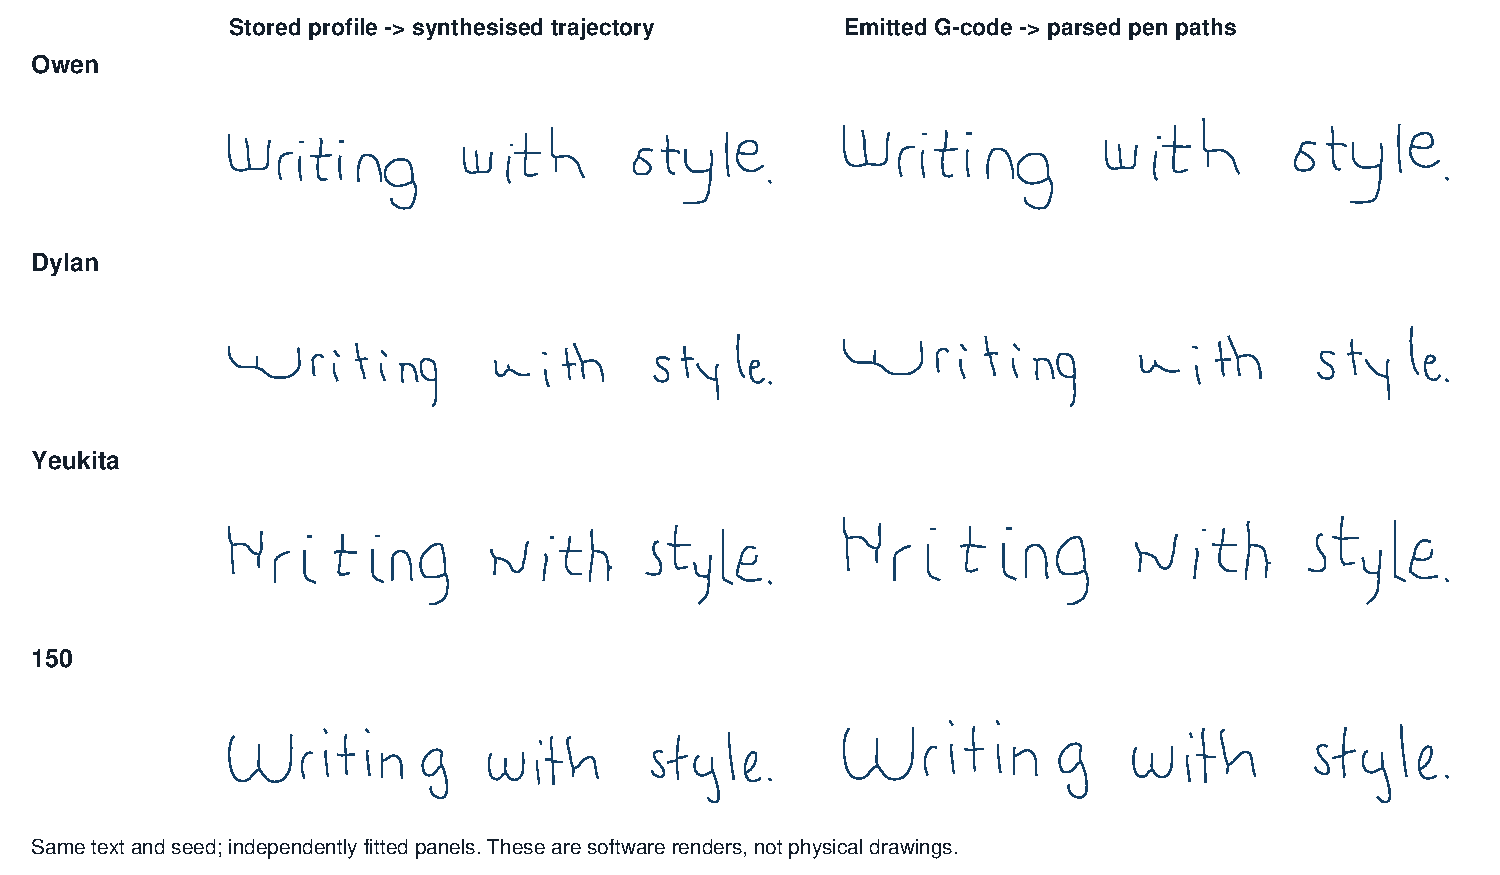
\includegraphics[width=0.98\linewidth]{Figures/design-style-gcode-examples.pdf}
\caption{Same text generated from four final profiles and reconstructed from emitted G-code. These are software path drawings.}
\label{fig:des-style-files}
\end{figure}

Algorithm~\ref{alg:des-file-reference} describes the serialization check. Nine controlled fixtures combined scale factors 1, 3 and 30 with line offsets 0, 8.4 and 25.2\,mm. Ring closure and joining were disabled, minimum-segment filtering was set to zero, and the independently parsed paths were paired with \texttt{ToMachine}'s output. Each fixture retained path and vertex counts, with no clamped points. Maximum coordinate error was $0.0004$\,mm, within the $0.0005$\,mm per-coordinate rounding bound from three-decimal emission. This comparison checks serialization after placement; it does not independently prove that the placement equation itself is correct or that a motor reached a coordinate.

\begin{designalgorithm}
\caption{Controlled G-code serialization correspondence}
\label{alg:des-file-reference}
\prequire{Known multi-path trajectory and configurations with joins and closure disabled.}
\begin{designpseudo}
\pstate{0}{\textbf{for each} fixture configuration $c$ \textbf{do}}
\pstate{1}{$P\leftarrow\operatorname{ToMachine}(T,c)$}
\pstate{1}{$f\leftarrow\operatorname{WriteGcode}(T,c)$; $Q\leftarrow\operatorname{ParseGcode}(f)$}
\pstate{1}{Compare path counts and corresponding vertex counts}
\pstate{1}{Record $\max_i\|P_i-Q_i\|_\infty$ and clamped-point count}
\pstate{0}{\textbf{end for}}
\pstate{0}{\textbf{return} count agreements, rounding discrepancies and clipping records}
\end{designpseudo}
\end{designalgorithm}

Figure~\ref{fig:des-physical-page} is separately identified as a photograph of actual robot output, from the existing Owen reproduction sheet. The line crops are newly obtained from that stored photograph. This closes the visual explanation from a physical page to the segmentation interface, without presenting the earlier drawing as a newly executed hardware experiment. No exact same-job correspondence with Figure~\ref{fig:des-style-files} is claimed.
\begin{figure}[!htbp]\centering
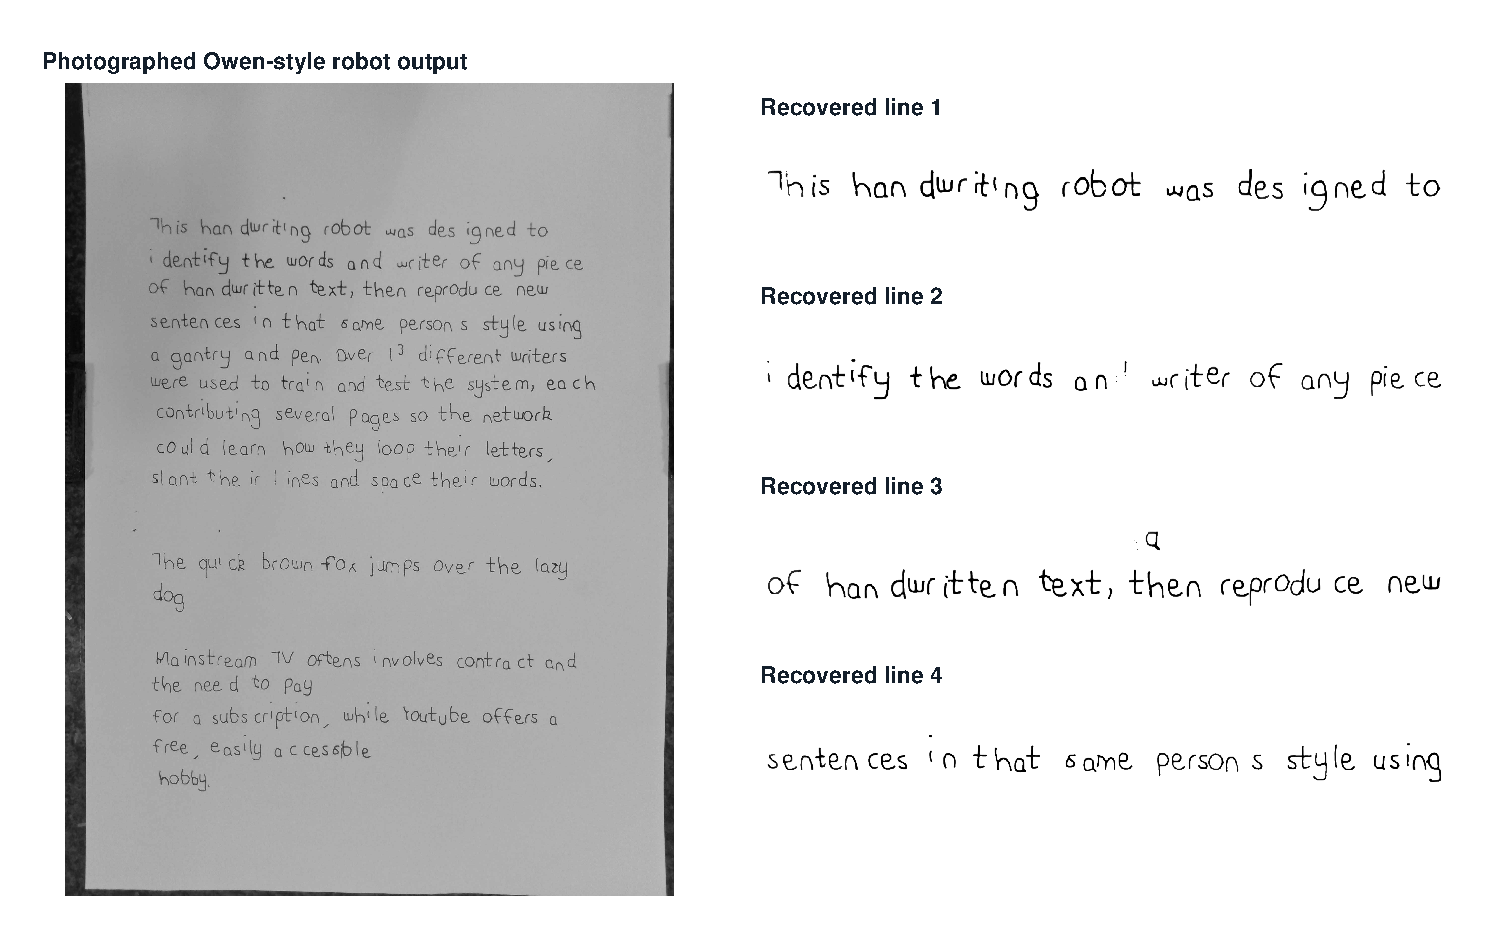
\includegraphics[width=0.95\linewidth]{Figures/design-physical-page-example.pdf}
\caption{Existing photographed robot output and newly recovered line crops. The photograph is distinct from the software renders above.}
\label{fig:des-physical-page}
\end{figure}

\subsection{Candidate-scoring configuration and scope}
The three Owen trials in Figure~\ref{fig:des-candidates} use the joint reader and selected \texttt{author\_shape\_11\_pw170\_weights.npz} model. Candidate images are rendered with uniform ink, then stroke-normalised explicitly at width 0.17 before writer inference. The bench selects both checkpoints and preprocessing explicitly. The diagnostic score uses the implemented character-accuracy function and requested-writer posterior before repair. The exact readings and full-precision scores are retained in \texttt{Evidence/bench.json}.
\FloatBarrier
